%==============================================================================
%  FORGE: A contract-driven framework for reusable hardware integration and
%         verification.
%
%  Drafted for submission to Open Research Europe (ORE) as a SOFTWARE TOOL
%  ARTICLE. ORE runs on the F1000Research platform; the section order below
%  (Introduction, Methods, Use cases, Discussion, availability and
%  author information) follows a software-tool article structure.
%
%  The framework core is algorithm- and domain-agnostic. The use cases are a
%  production trigger processor (the Phase-2 CMS OMTF) and the reference
%  consumers shipped with the framework (trigger_demo, vision_pipeline_demo,
%  passthrough_demo), which are the publicly reproducible part.
%
%  Figures live in figures/ as vector PDFs, each built from the matching
%  standalone TikZ source in the same directory (see figures/README.md for
%  the rebuild command). Rebuild a figure whenever you edit its .tex.
%  If you prefer ORE's official Overleaf template, paste the body sections
%  (Introduction onward) into it; the structure already lines up.
%
%  Compile with pdflatex -> bibtex -> pdflatex -> pdflatex.
%==============================================================================
\documentclass[10pt,a4paper]{article}

\usepackage[utf8]{inputenc}
\usepackage[T1]{fontenc}
\usepackage{lmodern}
\usepackage[a4paper,margin=2.3cm]{geometry}
\usepackage{microtype}
% Keep "--" as two hyphens in typewriter text, so inline CLI flags such as
% \texttt{--strict} print and copy correctly instead of as an en dash.
\DisableLigatures[-]{encoding=T1,family=tt*}
\usepackage{graphicx}
\usepackage{placeins}
\usepackage{xcolor}
\usepackage{booktabs}
\usepackage{tabularx}
\usepackage{array}
\usepackage{longtable}
\usepackage{listings}
\usepackage{enumitem}
\usepackage{authblk}
\usepackage{caption}
\usepackage{tikz}
\usepackage{amsmath}
\usetikzlibrary{arrows.meta,positioning,fit,backgrounds,calc,shapes.geometric}
\usepackage[colorlinks=true,allcolors=blue!55!black]{hyperref}
\newcolumntype{P}[1]{>{\raggedright\arraybackslash}p{#1}}
\newcolumntype{L}{>{\raggedright\arraybackslash}X}


\newcommand{\forge}{FORGE}
\newcommand{\hls}{HLS}


%---- palette -----------------------------------------------------------------
\definecolor{forgeblue}{HTML}{1F5C99}
\definecolor{forgebluelt}{HTML}{D6E4F0}
\definecolor{forgeorange}{HTML}{E2552B}
\definecolor{forgeorangelt}{HTML}{FBE2D8}
\definecolor{forgegray}{HTML}{5B6770}
\definecolor{forgegraylt}{HTML}{E7EAEC}
\definecolor{forgegreenlt}{HTML}{DDEBD8}
\definecolor{forgegreen}{HTML}{3F7D3F}

%---- listings style for YAML / CLI -------------------------------------------
\lstdefinestyle{forge}{
  basicstyle=\ttfamily\footnotesize,
  breaklines=true,
  columns=fullflexible,
  keepspaces=true,
  showstringspaces=false,
  frame=single,
  rulecolor=\color{forgegray!40},
  backgroundcolor=\color{forgegraylt!40},
  xleftmargin=4pt,xrightmargin=4pt,
  aboveskip=6pt,belowskip=6pt
}
\lstset{style=forge}
% Code blocks never split across pages: each listing is kept in one unbreakable box.
\lstnewenvironment{codeblock}[1][]
  {\endgraf\noindent\minipage{\linewidth}\lstset{#1}}
  {\endminipage\endgraf\vspace{4pt}}
\newcommand{\code}[1]{\texttt{\small #1}}

\captionsetup{font=small,labelfont=bf}

%==============================================================================
\title{\textbf{FORGE:} Framework for Orchestrated RTL Generation and Evaluation}

\author[1]{Pelayo Leguina}
\author[1]{Santiago Folgueras}
\affil[1]{Department of Physics, University of Oviedo, Oviedo, Spain}
\date{}

%==============================================================================
\begin{document}
\maketitle

%------------------------------------------------------------------------------
\begin{abstract}
A change to an FPGA module's ports can require edits to the structural RTL, port mappings, and testbench. FORGE (Framework for Orchestrated RTL Generation and Evaluation) resolves interface contracts and a declared topology into a design model. It generates structural RTL, testbench bindings, and board payloads, and sizes delays to align paths with different declared latencies. It can also simulate an existing RTL top and check its outputs against reference data. We tested FORGE on the Phase-2 Overlap Muon Track Finder (OMTF) of the CMS Level-1 trigger. The board design has 317 instances and 4357 connections. FORGE sized twelve delays to balance four merge points. In six board-payload simulations with an earlier FORGE revision, all 602 muons matched the emulator in transverse momentum, pseudorapidity, and azimuth. Two public examples show how to verify an unmodified CMS track-finder module and trace a deliberate error in a separate payload to its event and output link.
\end{abstract}

\vspace{0.5em}
\noindent\textbf{Keywords:} hardware framework; contract-driven design; FPGA;
high-level synthesis; design verification; reusable infrastructure;
clock-domain crossing; register-transfer-level simulation.

\vspace{1em}
\noindent\rule{\linewidth}{0.4pt}
\small
\noindent\textbf{Corresponding author:} Santiago Folgueras
(\href{mailto:folguerassantiago@uniovi.es}{folguerassantiago@uniovi.es}).
\normalsize
\vspace{1em}

%==============================================================================
\section{Introduction}
\label{sec:intro}

An FPGA payload can combine handwritten RTL with cores produced by high-level synthesis (HLS) or other generators. The structural top connects these modules to buffers, clock-domain-crossing logic, and board interfaces. The testbench must use the same ports and connections.

Module-level tests can miss integration errors such as a reset wired with the wrong polarity or two paths arriving at a merge in different cycles. HLS can also rename ports or change how an interface is represented in RTL. A single change can then require edits to the top level, testbench bindings, source lists, and simulation scripts.

IP-XACT provides a standard representation of IP interfaces and interconnections~\cite{IEEE_IPXACT_1685_2022}. Vivado IP integrator assembles and validates block designs through its graphical editor or Tcl~\cite{AMD_Vivado_IPI_UG994}. FORGE emits Tcl for IP integrator and can generate a structural Verilog top for simulation from the same design description. FuseSoC and Edalize package IP and run EDA tools~\cite{Kindgren2019_FuseSoC}.

FORGE (Framework for Orchestrated RTL Generation and Evaluation) is a Python tool for integrating and verifying FPGA modules. An interface contract maps the physical ports of a module to roles, such as a primary clock, reset, or data input. The topology connects instances through these roles or explicit port maps. FORGE resolves both descriptions into an intermediate representation (IR) for generation and analysis. It can also compare an existing RTL top with a reference using the top's sources and interface metadata.

We tested \forge{} on the Phase-2 Overlap Muon Track Finder (OMTF) of the CMS Level-1 trigger~\cite{CMS_2020_L1TriggerUpgrade_TDR} and on examples and reference consumers distributed with the source. Readers can rerun the public examples. For OMTF, we report results derived from the CMS collaboration's firmware and CI records.

\section{Methods}
\label{sec:methods}

\subsection{Implementation}
\label{sec:methods:implementation}

\subsubsection{Design description and structural generation}
\label{sec:forge:architecture}
\label{sec:forge:contract-model}

The module registry lists the modules and their build recipes. Each module's interface contract maps physical ports to roles, and the topology names the instances and connects them. \forge{} validates these inputs and resolves them into an IR with a versioned schema (Figure~\ref{fig:forge:architecture}). The generators and latency checker read this IR. To verify an existing top, \forge{} can work directly from its RTL sources and reference data.

\begin{figure}[!htb]
  \centering
  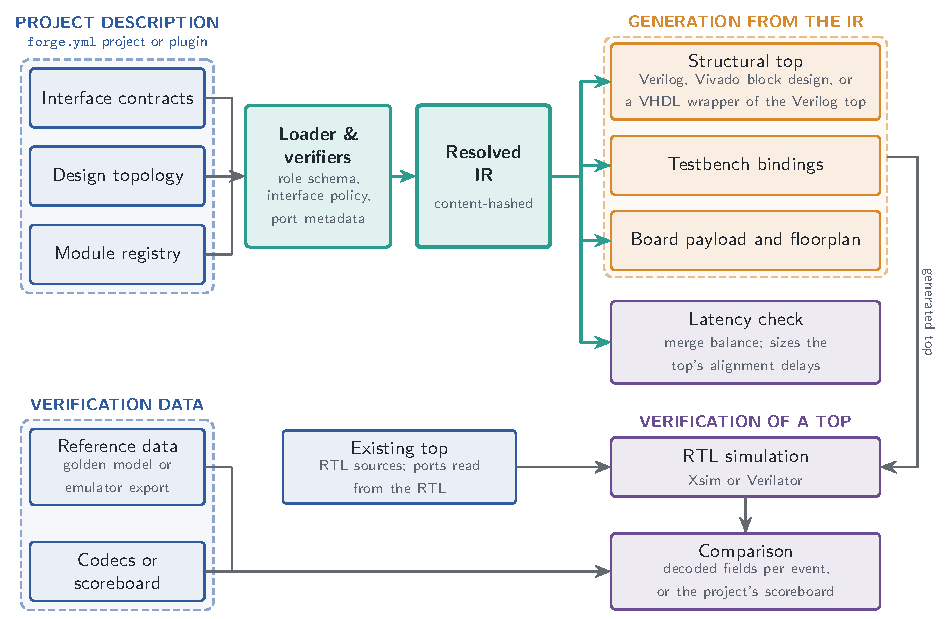
\includegraphics{figures/fig_forge_architecture}
  \caption{Design generation and RTL verification. Above, \forge{} resolves the design, generates the structural top, testbench bindings, and board payload, and sizes the alignment delays. Below, the simulator runs a generated or existing top. The verification flow compares its outputs with reference data using project codecs or a scoreboard.}
  \label{fig:forge:architecture}
\end{figure}

This excerpt from the \texttt{hit\_collector} contract in \texttt{trigger\_demo} shows the reset and four-element input array.

\begin{codeblock}
module_name: hit_collector
roles:
  reset_primary:
    raw_port: ap_rst
    direction: input
    width: 1
    active_level: high
  input_hit_array:
    array: true
    raw_port_prefix: in_hit_
    count: 4
    direction: input
    width: 32
    wiring_kind: decoded_hit
\end{codeblock}

The array expands to \texttt{in\_hit\_0} through \texttt{in\_hit\_3}. The \texttt{wiring\_kind} field connects it to a wiring family in the topology. The project defines its own role, \texttt{input\_hit\_array}. The common roles are listed in \texttt{canonical\_roles.yaml}. If HLS renames \texttt{ap\_rst}, the developer updates \texttt{raw\_port} in the contract. The topology refers to the role \texttt{reset\_primary}.

The generator uses the primary clock and reset roles to wire modules to their declared domains. Contract verification reports a missing primary clock or reset role as an error unless the module is declared clock-free or reset-free; structural generation reports the same omission as a warning. Validation also compares role directions, widths, and array lengths with the port metadata.

Before HLS, \forge{} predicts the ports from C++ signatures and pragmas. After synthesis it can read the actual ports from the RTL. Some AXI bundles and padded structures depend on synthesis decisions and can remain unresolved. The IR records whether each interface is parsed, predicted, synthesized, reconciled, or verified. Projects can declare vendor IP and encrypted blocks as opaque modules and wire their secondary clocks and resets individually.

The topology connects instances through role families, explicit port maps, or contract wirings. Two emitters write the resolved topology as structural Verilog or as a Vivado IP-integrator block design; a VHDL option wraps the Verilog top in a VHDL entity and has not been carried through a downstream flow. With \texttt{--strict}, generation fails if any output is left open or any input tied off without a declaration. \texttt{forge inspect} exports the resolved IR as JSON with its content hash, and \texttt{forge inspect --impact} compares two resolved designs and lists the merge points a change misaligns.

\subsubsection{Latency and clock-domain crossings}
\label{sec:forge:latency}
\label{sec:forge:cdc}

The latency analyzer builds a directed graph of instances and connections. A module's latency is taken from an explicit registry declaration, then from an HLS synthesis report~\cite{AMD_VitisHLS_UG1399}, then from a manual hint; otherwise it remains unknown. For a single-clock merge point $m$ with known incoming path latencies $L(p_1),\ldots,L(p_k)$, the checker computes
\[
\Delta(m)=\max_i L(p_i)-\min_i L(p_i),
\]
and the paths are balanced when $\Delta(m)=0$. A connection declared \texttt{delay\_cycles: auto} receives the delay that brings its arrival to the latest arrival at the merge point, sized in topological order and recorded in the build manifest. Generation stops if \forge{} cannot resolve a delay, for example when a path latency is unknown or the merge lies on a feedback loop. The checker reports a late fixed input as a mismatch and leaves its delay unchanged. A connection declared \texttt{static: true}, such as a configuration word written before the data it configures, stays in the graph but takes no part in alignment. For bounded latencies, the checker looks for overlap between arrival intervals at the merge point. Framed merges align by record boundaries. Elastic paths have no fixed cycle alignment. Figure~\ref{fig:forge:latency} shows an exact-cycle and a bounded merge of the platform-wrapper design of Section~\ref{sec:forge:use-cases:vision}.

\begin{figure}[!htb]
  \centering
  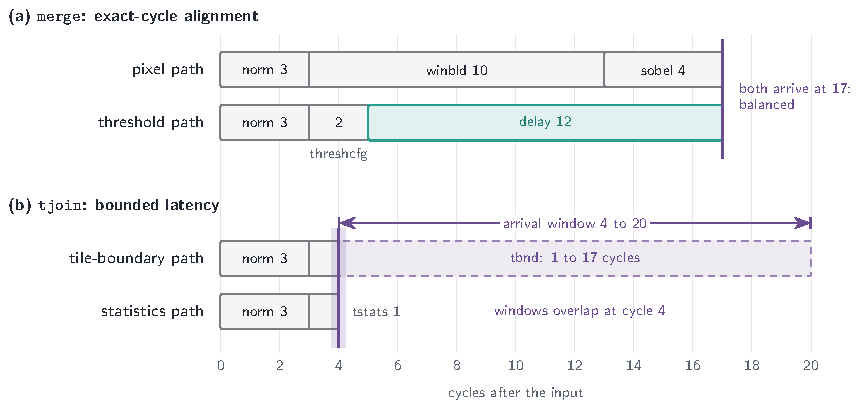
\includegraphics{figures/fig_forge_latency}
  \caption{Arrival times at two merges in the platform wrapper. (a) Both paths reach \texttt{merge} at cycle 17. The threshold path uses a fixed 12-cycle delay, which is also the delay \forge{} would select automatically. (b) The tile-boundary path reaches \texttt{tjoin} between cycles 4 and 20. That interval includes the statistics path's arrival at cycle 4.}
  \label{fig:forge:latency}
\end{figure}

A connection between clock domains must declare an adapter: a two-flop level synchronizer, a pulse synchronizer, a mailbox handshake, or an asynchronous FIFO, whose RTL \forge{} emits, or a waiver with a reason. An undeclared crossing stops generation. The latency graph adds two destination-clock cycles for a level synchronizer and three for a pulse synchronizer; mailbox and FIFO transfer times remain unknown. The checker uses declared latencies and keeps cycle counts from different clock domains separate. RTL latency, physical timing, and metastability require separate checks.

Static throughput analysis estimates the nominal capacity $rf/\mathrm{II}$ of a stage that accepts $r$ records per initiation interval at frequency $f$. A simulation probe samples FIFO status on one clock and reports occupancy and the average rate over the sampled interval. For multi-clock or enable-gated FIFOs, the project must count the transactions separately.

\subsubsection{Verification}
\label{sec:forge:verification}

For a \texttt{forge.yml} project, \texttt{forge test} reads the top name, clock, reset, RTL sources, and input and expected data. For link words, codecs can specify which bits encode each field. \forge{} reads the RTL ports, drives the inputs, and compares the specified output fields in each event, in order or as a set. The report gives the event, interface, cycle, and fields that differ. It records a missing packet against the event in which it was expected. Use \texttt{--event-id} to replay a single event. The testbench drives and reads HLS memory interfaces through the HLS memory protocol.

A plugin declares its verification flows for HLS C simulation, individual RTL modules, and the integrated payload. The RTL flows use a generated SystemVerilog testbench whose port bindings come from the current interface metadata. A flow may keep a hand-written port map, and \texttt{forge dev verify generate} compares its ports, directions, and widths with the RTL and stops if they disagree. The plugin interprets the dataset and supplies the reference-model provider and scoreboard. \forge{} invokes the provider, records hashes of the input and output, and runs the flow. RTL simulation uses AMD Xsim~\cite{AMD_Vivado_LogicSimulation_UG900} or Verilator. This infrastructure can host methodologies such as UVM~\cite{Accellera_UVM} but does not provide constrained-random stimulus or coverage closure. \texttt{forge report} collects topology, latency, throughput, and verification results into an offline HTML report without rerunning them.

\subsubsection{Board frameworks and existing projects}
\label{sec:forge:external-integration}
\label{sec:forge:core-isolation}

The \texttt{framework} commands load an external board framework's ABI and endpoint manifests and emit the payload wrapper around the generated top, matching links from manifest data. What a board needs beyond per-link wiring is declared as payload control policies rather than patched into the generated file: input and output registers, receive gates, configuration and status words mapped to framework registers, and the project's own Verilog blocks. A floorplan command assigns block-design cells to device regions from the resolved links. For an existing repository, \texttt{forge init} writes a minimal \texttt{forge.yml} and \texttt{forge adopt} scans sources and the instantiation graph, recording the decisions the scan cannot make; the adoption commands are covered by repository tests, and no third-party adoption is evaluated here. Commands that accept \texttt{--json} return a common envelope of status, diagnostics, artifacts, and metrics, with exit code 0 for a pass, 1 for a failure or a warning under \texttt{--strict}, and 2 for usage or internal errors.

\subsection{Operation}
\label{sec:methods:operation}

\subsubsection{System requirements}

\forge{} is an MIT-licensed Python package, version~3.0.0, with a \texttt{forge} command-line entry point. It requires Python~$\geq3.8$~\cite{Python_Language}, PyYAML~\cite{PyYAML}, and Jinja2~\cite{Jinja2}. Contract validation, structural generation, and static analysis do not invoke vendor tools. HLS synthesis and C simulation require Vitis HLS. The block-design output targets Vivado IP integrator. For RTL simulation, Xsim and Verilator are supported. Waveform and probe capture are available with Xsim. The main set of archived experiments used Linux, Python~3.9.25, PyYAML~6.0, Jinja2~3.1.6, Vitis HLS and Vivado~2024.1, and Verilator~5.022.

\subsubsection{A runnable example}
\label{sec:methods:implementation:workflow}

The \texttt{examples/cmssw\_reference} directory of the source contains a 100-event export of the CMS OMTF emulator, two codecs, and a small payload, \texttt{candidate\_to\_gmt.v}, that rewrites each link's track-finder candidates as Global Muon Trigger words. Its \texttt{forge.yml} is the complete description:

\begin{codeblock}
project: cmssw_reference
top: candidate_to_gmt
sources:
  rtl: [rtl/*.v]
clock: {port: clk}
reset: {port: rst, active: high}
verification:
  target: existing
  backends: [verilator, xsim]
  input: {path: data/input.txt, format: empv2, events: data/input.events.json}
  expected: {path: data/expected.txt, format: empv2, events: data/expected.events.json,
             provenance: data/provenance.json}
  links: {l0: 0, l1: 1, l2: 2, l3: 3, l4: 4, l5: 5, q0: 0, q1: 1, q2: 2, q3: 3, q4: 4, q5: 5}
  codecs:
    "q*": codecs/samuon.yml
  compare: {fields: [pt, eta, phi, charge, qual], order: event}
\end{codeblock}

With FORGE v3.0.0 installed, run these commands from the example directory to pack the export into pattern files, simulate the top, and write the report:

\begin{codeblock}
python3 make_patterns.py   # data/input.txt: 100 events, 217 candidates
forge test                 # Verilator and Xsim, whichever is installed
forge report               # .forge/reports/verification_results.md
\end{codeblock}

The Verilator result reports the number of matched and expected words on each link:

\begin{codeblock}[basicstyle=\ttfamily\scriptsize]
existing:candidate_to_gmt [verilator]: VERIFIED (q0 32/32, q1 35/35, q2 43/43, q3 38/38, q4 33/33, q5 36/36)
\end{codeblock}

To adapt the example, supply the new RTL and its reference export, and update the codecs and port mappings to match the design.

\section{Use cases and validation}
\label{sec:forge:use-cases}

\subsection{Public examples}
\label{sec:forge:use-cases:golden-path}

We ran the CMS emulator example from Section~\ref{sec:methods:implementation:workflow} in Xsim and Verilator. On all six links, the decoded fields of all 217 output muons matched the CMS emulator export event by event. This checks the payload's conversion between two link-word formats.

We added one to every output muon's \texttt{eta} field and reran the example in Verilator. All 217 output words differed from the reference, each in \texttt{eta} alone. The first mismatch was on link \texttt{q0}:

\begin{codeblock}
q0, event 2, index 0, cycle 4: expected eta=1246, observed eta=1247 (valid, charge, pt, phi, d0, qual equal)
\end{codeblock}

\noindent Running \texttt{forge test --backend verilator --event-id 2} reproduced the mismatches for the two muons in that event, one on \texttt{q0} and one on \texttt{q5}. The archive includes the patch and the records from both runs.

For the second example, we simulated the CMS Level-1 track finder's VMRouter~\cite{L1TK_firmware_hls} without changing its RTL. \forge{} drives the input memories and reads the output memories using the HLS memory protocol. In Xsim, all 938 AllStub words and 938 ME stubs matched the emulation printouts over 100 events. The example uses Vitis HLS and Vivado~2024.1 and downloads test vectors from the track-finder project.

\subsection{The Phase-2 OMTF trigger processor}
\label{sec:forge:use-cases:omtf}

The Overlap Muon Track Finder reconstructs muon candidates where the CMS barrel and endcap muon systems overlap, from the stubs of drift tubes, cathode strip chambers, and resistive plate chambers. Its Phase-2 implementation for the Level-1 trigger~\cite{CMS_2020_L1TriggerUpgrade_TDR} targets an X2O board with a Virtex UltraScale+ VU13P and a 360\,MHz algorithm clock (nine cycles per 25\,ns bunch crossing). The processor has fixed latency. It receives 85 detector links, sends its candidates to the Global Muon Trigger on 18 output links, and uses the CMSSW OMTF emulator as its reference.

\begin{figure}[!htb]
  \centering
  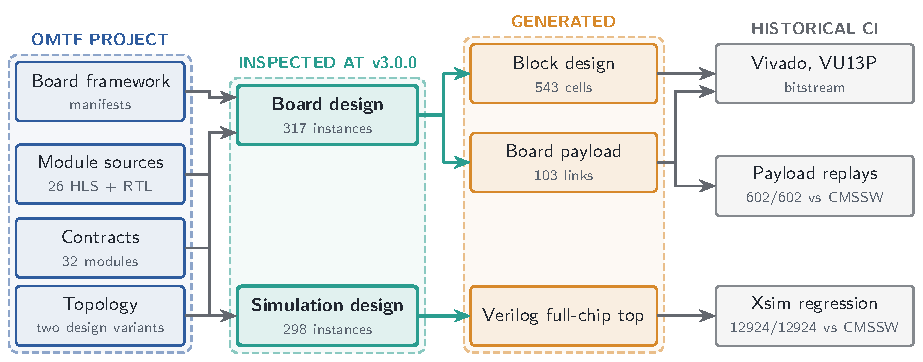
\includegraphics{figures/fig_forge_omtf}
  \caption{Board and simulation variants of OMTF. Vivado uses the board design and payload to build the bitstream. The payload replays and the full-chip Verilog regression compare outputs with the CMSSW emulator. The instance counts come from inspection with \texttt{v3.0.0}. Table~\ref{tab:forge:omtf} gives the revisions used for the CI runs.}
  \label{fig:forge:omtf}
\end{figure}

\paragraph{Design.}
The algorithm consists of 26 HLS modules, from the detector interfaces to the neural-network regression and output linking, and hand-written RTL for configuration samplers and pipeline delays. The project describes two variants (Figure~\ref{fig:forge:omtf}): the board design, with 32 modules, 317 instances, and 4357 connections, and a full-chip simulation design, with 30 modules, 298 instances, and 4038 connections, whose configuration words and output links are top-level ports instead of board-framework signals. In the board variant, all 32 modules have interface contracts. FORGE resolves the connections from 47 topology groups, 16 explicit port maps, and six contract wiring declarations without falling back to port-name matching. Both variants pass strict generation. Inspection warns that the two RPC link demultiplexers lack primary clock and reset declarations and have no exemption. The contract verifier treats these omissions as errors.

\paragraph{Latency.}
The detector branches take different numbers of cycles to reach four merge points. Using declared and HLS-reported latencies, \forge{} computes twelve delays of 2 to 73 cycles and reports all four merges as balanced. The topology requests these delays with \texttt{delay\_cycles: auto}. If resynthesis changes a module's latency, \forge{} recalculates the delays from the new reports. The board design marks 133 inputs as static, which keeps the configuration samplers out of the alignment calculation.

\paragraph{Board integration.}
The board framework supplies its ABI and endpoint manifests. \forge{} resolves the 85 input and 18 output links against them and generates the payload with the project's control policies: one register per input and output link, the replay control of the spy buffers, the lock on the bunch-crossing-zero marker, and 132 configuration words mapped to the framework's registers. The floorplan command assigns block-design cells to device regions. The project used the generated block design and payload to build a VU13P bitstream (Table~\ref{tab:forge:omtf}).

\paragraph{Verification against the emulator.}
The CI pipeline runs C simulation for 18 modules, exports the 26 HLS modules, and runs the full-chip regression. The regression matched the reference set in all 12924 output slots. A separate board-payload simulation loaded the spy buffers and replayed six sets of 100 events, one set for each processor and endcap side. All 602 muons matched the emulator in transverse momentum, pseudorapidity, and azimuth. The replay found no wrong or extra words and none outside the expected event slots.

The CI runs used earlier \forge{} revisions (Table~\ref{tab:forge:omtf}). With the same OMTF revision and HLS outputs, \texttt{v3.0.0} reproduces the Verilog tops and twelve alignment delays from \texttt{3a5bc03}, the revision used for the archived implementation.

\begin{table}[!htb]
  \centering
  \footnotesize
  \renewcommand{\arraystretch}{1.18}
  \caption{The OMTF design in \forge{}. Structure and latency from \texttt{forge inspect} and \texttt{forge dev analyze latency-check} at \texttt{v3.0.0}; the last three rows from the project's continuous integration at the commits shown.}
  \label{tab:forge:omtf}
  \begin{tabularx}{\textwidth}{@{}P{4.4cm}L@{}}
    \toprule
    Item & Value \\
    \midrule
    Board design & 32 modules, 317 instances, 4357 connections \\
    Simulation design & 30 modules, 298 instances, 4038 connections \\
    Contracts and wiring & Board variant: 32 of 32 modules have contracts, with no port-name matches \\
    Merge points; delays sized & 4, balanced; 12, from 2 to 73 cycles (both designs) \\
    Board payload & 85 input links, 18 output links, and 132 configuration words \\
    Archived VU13P implementation (\texttt{3a5bc03}) & Bitstream generated \\
    Payload replays (\texttt{03cf162}) & 6 sets of 100 events; 602 of 602 muons \\
    Regression (earlier revision) & 12924 of 12924 output slots \\
    \bottomrule
  \end{tabularx}
\end{table}

\subsection{A multi-clock image-processing pipeline}
\label{sec:forge:use-cases:vision}

The \texttt{vision\_pipeline\_demo} reference consumer contains 19 interface contracts and nine design variants, two of them invalid fixtures. Its platform-wrapper variant has 12 instances, 119 connections, and three clock and reset domains, and all 12 modules resolve through contracts. Figure~\ref{fig:forge:platform} is drawn from \forge{}'s own rendering of this design and from its archived latency report.

\begin{figure}[!htb]
  \centering
  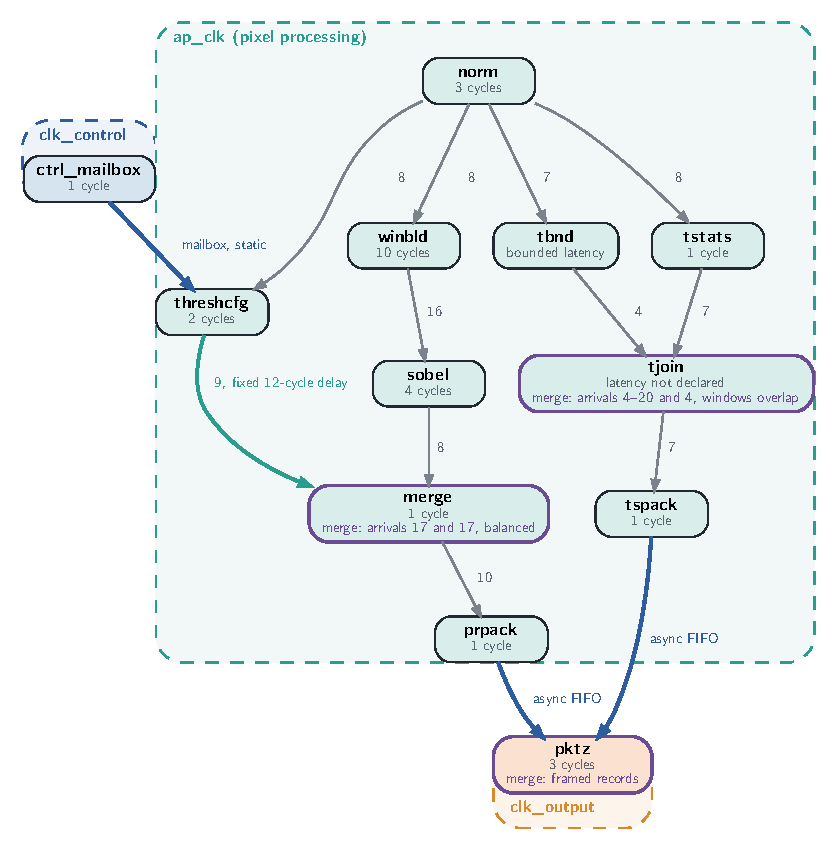
\includegraphics{figures/fig_forge_platform_wrapper}
  \caption{Platform wrapper drawn from \texttt{forge inspect --dot} and the latency report. Boxes show instances and their declared latencies. Colors group instances by clock domain. Edge labels count resolved connections, excluding clock and reset nets. Blue edges mark crossings and name their adapters. The green edge carries a fixed 12-cycle delay. Purple borders identify merges and their arrival times.}
  \label{fig:forge:platform}
\end{figure}
\FloatBarrier

The checker found no mismatches or unknown arrivals at the three merges. The pixel and threshold paths arrive at \texttt{merge} in the same cycle. At \texttt{tjoin}, the tile-boundary interval includes the statistics path's arrival (Figure~\ref{fig:forge:latency}). The packetizer takes framed records from two asynchronous FIFOs. The checker skips cycle alignment on those inputs. The threshold setting crosses domains through a mailbox. Its static declaration excludes it from alignment.

The CDC variant exercises six crossings using all four adapter kinds. In Xsim, all six checks of level status, pulse counts, and received data passed. All eight valid simulation flows passed. The scoreboard flagged an undersized FIFO with \texttt{pixel\_result\_record mismatch}. Strict generation rejected a direct bus between clock domains and reported the clock and reset domains involved.

\subsection{Validation record and reproducibility}
\label{sec:forge:results}

Table~\ref{tab:forge:results} summarizes the public results. The evidence collector reads the list of expected flows from the verification contracts. It checks complete logs for pass markers or the expected error for each invalid fixture. The trigger example includes C simulation, single-module RTL simulation, and an integrated payload test. The payload testbench waits up to 30 cycles for the output strobe and compares the response value.

\begin{table}[!htb]
  \centering
  \footnotesize
  \renewcommand{\arraystretch}{1.18}
  \caption{Results of the public examples and reference consumers, from the archived evidence. RTL simulation uses Xsim unless stated.}
  \label{tab:forge:results}
  \begin{tabularx}{\textwidth}{@{}P{4.0cm}L@{}}
    \toprule
    Item & Archived result \\
    \midrule
    CMS emulator example & 217 of 217 muons on six links, Xsim and Verilator \\
    Same, eta changed by one unit & 0 of 217 matched; every difference in eta (Verilator) \\
    VMRouter, unmodified & 938 of 938 ME and 938 of 938 AllStub words, 100 events \\
    Platform wrapper & 12 instances, 119 connections, 3 domains; 3 merges, no mismatch \\
    Vision simulations & 8 of 8 pass; both invalid fixtures rejected with their diagnostics \\
    CDC variant & 6 checks pass across the four adapter kinds \\
    Trigger consumer & 4 C-simulation, 4 single-module and 1 integrated RTL flow pass \\
    Framework test suite & 2417 passed, 12 skipped, with the EDA tools present \\
    \bottomrule
  \end{tabularx}
\end{table}

The evidence README records the tools, test skips, and packetizer measurements.

The reference-consumer logs come from one session on a clean checkout of the cited commit. The archive hashes the log files. Linking each log to the simulated executable would require per-flow build hashes. To reproduce the simulations, build and run the flows again. We ran the public example's negative control separately with Verilator~5.020.

\section{Discussion}
\label{sec:forge:conclusions}
\label{sec:forge:limitations}

The OMTF project used the same module contracts for its simulation top and board design. The project captured board-specific behavior in payload policies and gave FORGE the module latencies needed to calculate alignment delays. Measuring the effect on engineering effort would require comparing how developers handle the same integration and maintenance tasks with another workflow.

The public examples use existing RTL and reference data, so readers can reproduce the comparisons and replay the injected error. The OMTF evidence is limited to reports derived from simulation and implementation with restricted CMS inputs.

The latency checker keeps clock domains separate and checks a bounded latency at the merge it reaches. It does not propagate the interval through later stages. The CDC simulation covers the transfers in the reference test. Other clock ratios and traffic patterns require further tests, and metastability requires a separate assessment. The throughput probe infers transfers from FIFO status sampled on one clock. A sustained-load measurement would need handshake counters sampled in each domain.

The generator regression compares the IR-based and earlier generation paths on two reference designs. Reference simulations compare the outputs against project data. The VHDL wrapper still needs downstream validation. The common vocabulary retains synchronization, cycle-counter, and reference-hit roles from bunch-crossing trigger designs. Projects can define their own roles, and the source check rejects detector names in the framework packages. An evaluation in other projects should record where the common roles suffice and where developers need project-specific contracts.

%==============================================================================



%==============================================================================
\section*{Data availability}
%==============================================================================
The cited \forge{} revision includes the public examples, reference datasets, and expected outputs~\cite{FORGE_Software}. The article repository contains the logs, run records, and derived reports cited in Section~\ref{sec:forge:use-cases}. The evidence README documents anonymization, and the validation script checks file hashes and recorded outcomes. Access to the OMTF firmware, CMS emulator reference sets, and CI records is restricted to CMS collaboration members. The article repository contains the derived OMTF reports and their hashes (Section~\ref{sec:forge:use-cases:omtf}). The archive excludes raw probe traces, HLS build directories, and board measurements.

\section*{Software availability}
\label{sec:forge:software-availability}

\forge{} is distributed under the MIT license at
\url{https://github.com/pleguina/forge}. The source revision associated with this article is
release \texttt{v3.0.0}, commit \texttt{90ff3450157359b6abe78c97ee98cce1c345ec95}.
% TODO before submission: deposit the v3.0.0 release with a DOI (Zenodo GitHub integration) and cite it.
The package declares Python~$\geq3.8$, PyYAML, and Jinja2 as requirements.
Reference consumers and their tests are included under \texttt{plugins/} and
\texttt{forge/tests/}. The article sources and evidence bundle are maintained at
\url{https://github.com/pleguina/forge_paper}. A release archive with a persistent
identifier has not yet been deposited. The archived evidence and its limitations
are described in Section~\ref{sec:forge:results}.

\section*{Author contributions}
%==============================================================================
P.\ Leguina and S.\ Folgueras jointly designed the framework architecture and
contract model, implemented the tooling and verification runtime, and wrote the
manuscript.

\section*{Competing interests}
The authors declare no competing interests.

\section*{Grant information}
This work is supported by ERC grant (INTREPID, 101115353, \href{https://doi.org/10.3030/101115353}{10.3030/101115353}). Funded by the European Union. Views and opinions expressed are however those of the author(s) only and do not necessarily reflect those of the European Union or the European Research Council Executive Agency. Neither the European Union nor the granting authority can be held responsible for them.

\section*{Acknowledgements}
The authors thank early users of the framework's reference consumers for
feedback that shaped the command-line workflow and the core-isolation
checks described in this article.

%==============================================================================
%  References. ORE uses a numbered Vancouver-style reference list.
%==============================================================================
\bibliographystyle{vancouver} % Standard Vancouver-like sequential numerical style
\bibliography{references}   % Name of your references.bib file

\end{document}
